\chapter{Appendix}
\section{Study the Upper bound in Python}
The following code shows how we estimated an upper bound in symmetric critical arcgons. result\_positve, result\_negative and result\_zero are three functions we developed to calculate the stretch factor when $x$ and $k$ are given. Then, we first use the function called less\_than to check if all cases with negative  $k$ is not worse than those with $k=0$. Then, by testing the stretch factors between a relatively small steps in $k$'s, we could provide an upper bound by showing the existence of a arcgon with such stretch factor.



\begin{minted}[breaklines]{python}
from numpy import *


# find X in (l, r) based on gamma
def findX(gamma, l, r):
	mid = l + (r-l)/2
	diff = mid + arcsin(mid) - pi/2 + gamma
	if fabs(diff) <= 0.00001:
		return mid
	elif diff > 0:
		return findX(gamma, l, mid)
	else:
		return findX(gamma, mid, r)



# calculate the stretch factor when k is positive, negative or zero
def result_positive(x, k):
	path = pi/2 - arcsin(x) + sqrt(k**2+x**2)*arctan(x/k)
	distance = (sqrt(1-x**2)-k)*cos(x) + sqrt(k**2+x**2)*cos(x/sqrt(k**2+x**2)-x)
	return path/distance

def result_negative(x, k):
	path = pi/2 - arcsin(x) + sqrt(k**2+x**2)*(pi - arctan(x/k))
	distance = (sqrt(1-x**2)+k)*cos(x) + sqrt(k**2+x**2)*cos(x/sqrt(k**2+x**2)-x)
	return path/distance

def result_zero(x):
	path = pi/2 - arcsin(x) + x*pi/2
	distance = sqrt(1-x**2)*cos(x) + x*cos(1-x)
	return path/distance


# check if all cases of negative k less than the cases that k=0
def check_less_than(list, kl, kr):
	for x in list:
		zero = result_zero(x)
		k = kl
		while k < kr:
			res = result_negative(x, k)
			if res > zero:
				print 'FAIL', x, '-', k
			k = k + 0.001
	print 'SUCCESS'

def less_than(size):
	list = []
	for num in xrange(1, size+1):
		list.append(num*0.739/size)
	check_less_than(list, 0.001, 1)



# find the maximun stretch factor by scanning all k's
def local_max(list, kl, kr):
	ans = []
	for gamma in list:
		subans = [gamma, 0, 0, 0]
		worst = 0
		k = kl
		while k < kr:
			res = result_positive(gamma, k)
			if res > worst:
				worst = res
				subans[1] = findX(subans[0], 0.0, 1.0)
				subans[2] = k
				subans[3] = res
			k = k + 0.00001 
		ans.append(subans)
	return ans

# find the maximun stretch factor by scanning all gamma
def local_max2(list, gl, gr):
	ans = []
	for k in list:
		subans = [k, 0, 0, 0]
		worst = 0
		g = gl
		while g < gr:
			res = result_positive(g, k)
			if res > worst:
				worst = res
				subans[1] = findX(g, 0.0, 1.0)
				subans[2] = g
				subans[3] = res
			g = g + 0.001 
		ans.append(subans)
	return ans
\end{minted}

We also the similar strategy on symmetric critical arcgons with more than three circles. The code below is how we implement the case with five base circles. Figure~\ref{fig:k1k2} shows the trend of stretch factors with varied $k_1$ and $k_2$. 










\begin{minted}[breaklines]{python}
import matplotlib.pyplot as plt
from numpy import *
from mpl_toolkits.mplot3d import Axes3D

# find X in (l, r) where gamma = 0
def findX1(l, r):
	mid = l + (r-l)/2
	diff = mid + arcsin(mid) - pi/2
	if fabs(diff) <= 0.000000001:
		return mid
	elif diff > 0:
		return findX1(l, mid)
	else:
		return findX1(mid, r)


# find X2 in (l, r) where gamma = 0
def findX2(k1, l, r):
	mid = l + (r-l)/2
	diff = x1 + mid - sqrt(k1**2+x1**2)*arctan(x1/k1) + sqrt(k1**2+x1**2)*arcsin(mid/sqrt(k1**2+x1**2))
	if fabs(diff) <= 0.000000001:
		return mid
	elif diff > 0:
		return findX2(k1, l, mid)
	else:
		return findX2(k1, mid, r)


# find the raduis r given k and x
def update_r(k, x):
	return sqrt(k**2+x**2)


# calculate the stretch factor, where k, t could only be positive (used in array calculation in 3d_plot)
def result_positive(k1, k2):
	x2 = findX2(k1, 0.0, 1.0)
	r1 = update_r(k1, x1)
	r2 = update_r(k2, x2)
	path = x1 + r2*arctan(x2/k2) + r1*(arctan(x1/k1)-arcsin(x2/r1))
	distance = ((sqrt(1-x1**2)-k1)*cos(x1) 
		+ (sqrt(r1**2-x2**2)-k2)*cos(arctan(x1/k1) - x1 - arcsin(x2/r1)) 
		+ r2*cos((1-r1/r2)*arctan(x1/k1) +(1/r2-1)*x1 + arccos(x2/r1) - arctan(k2/x2) + (r1/r2)*arcsin(x2/r1) - arctan(x2/k2))
	)
	return path/distance


# return the worest cases for each gamma in list
def local_max(k1l, k1r, k2l, k2r):
	ans = []
	worst = 0;
	k1 = k1l
	while k1 <= k1r:
		k2 = k2l
		x2 = findX2(k1, 0.0, 1.0)
		k2r = sqrt(k1**2+x1**2-x2**2)
		while k2 <= k2r:
			res = result_positive(k1, k2)
			subans = [x1, findX2(k1, 0.0, 1.0), k1, k2, res]
			ans.append(subans)
			if (res > worst):
				worst = res
			k2+=0.01
		k1+=0.01
	print 'worst '+str(worst)

	return ans

# return a 2D graph to show relationship btw SF and gamma by size many dots
def two_dim_plot():
	list = [0.1, 0.2, 0.3, 0.4, 0.5, 0.6]

	for num in range(6):
		y = local_max(list[num], list[num], 0.01, 1)
		max1 = []
		max2 = []
		for arr in y:
			max1.append(arr[3])
			max2.append(arr[4])

		plt.subplot(2, 3, num+1)
		plt.plot(max1, max2, 'o-')
		plt.title('k1 = '+ str(list[num]))
		plt.xlabel('k2')
		plt.ylabel('Stretch Factor')
	plt.show()

two_dim_plot()
\end{minted}

\begin{figure}[ht]
\centering
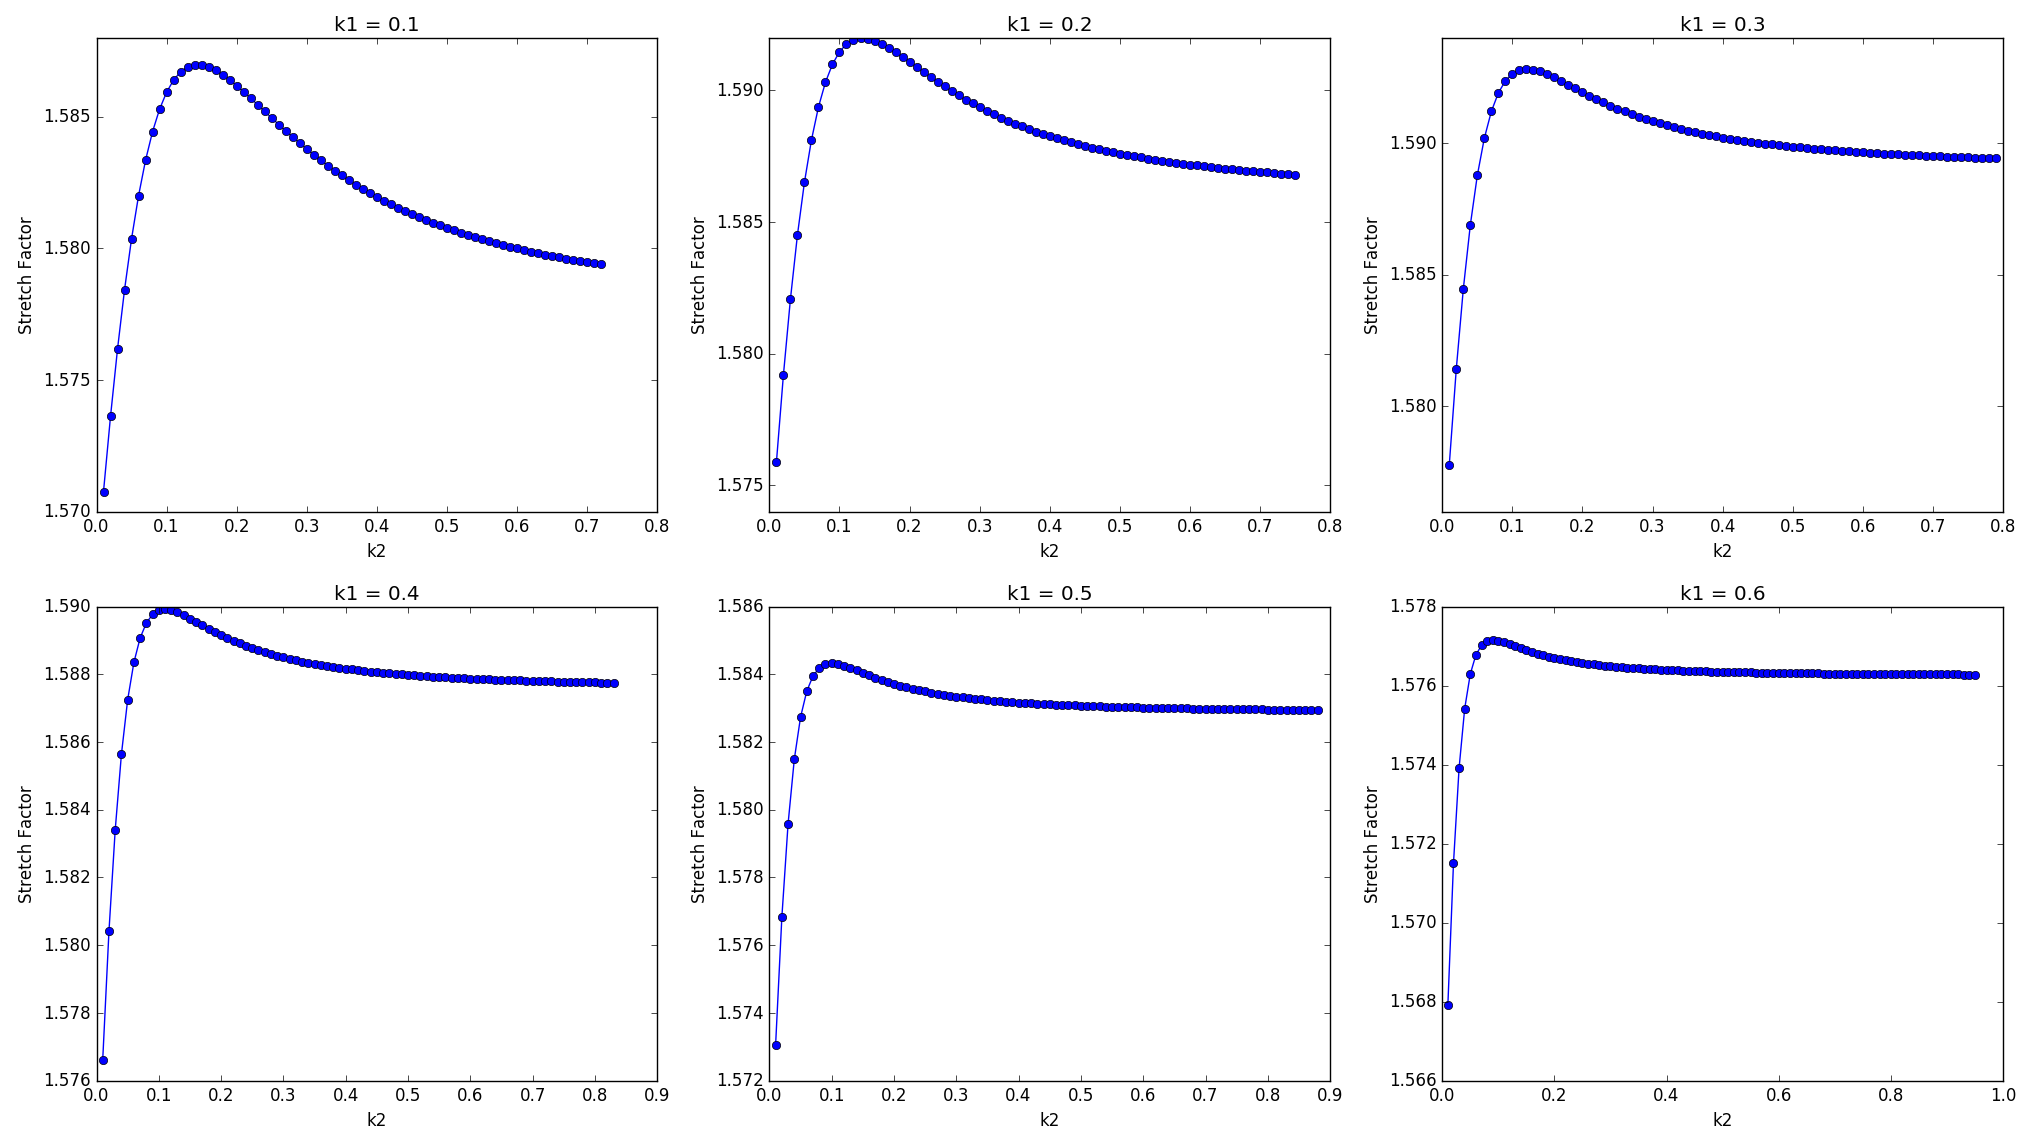
\includegraphics[width=\textwidth]{Figures/k1k2.png}
\caption[Constrained Delaunay triangulation in path planning in Automated driving]{Constrained Delaunay triangulation in path planning in Automated driving.} 
\label{fig:k1k2}
\end{figure}




\section{Study the Lower bound in Python}
As we discussed in Chapter 6, to improve the lower bound of the stretch factor in arcgons, we first calculate the partial derivatives in both $x$ and $k$ directions. Then, simulate recursively on the stretch factors of every block so that the maximun possible stretch factors based on the partial derivatives is still less than our target value, $1.6$. The following python code is our implementation of this simulation.
\begin{minted}[breaklines]{python}
from sympy import *

# Generate the partial derivatives of func f
x = Symbol('x');
k = Symbol('k');

path = 1.5707963267949 -asin(x) + sqrt(k**2+x**2)*atan(x/k)
distance = (sqrt(1-x**2)-k)*cos(x) + sqrt(k**2+x**2)*cos(x/sqrt(k**2+x**2)-x)
f = path/distance
diff_x = diff(f, x)
diff_k = diff(f, k)

print diff_x
print diff_k


# calculate the stretch factor given x and k
def func(x, k):
	path = 1.5707963267949 -asin(x) + sqrt(k**2+x**2)*atan(x/k)
	distance = (sqrt(1-x**2)-k)*cos(x) + sqrt(k**2+x**2)*cos(x/sqrt(k**2+x**2)-x)
	return path/distance

# find the partial derivative with respective to x
def pdiff_x(x, k):
	diff_x = (x*atan(x/k)/sqrt(k**2 + x**2) - 1/sqrt(-x**2 + 1) + sqrt(k**2 + x**2)/(k*(1 + x**2/k**2)))/((-k + sqrt(-x**2 + 1))*cos(x) + sqrt(k**2 + x**2)*cos(x - x/sqrt(k**2 + x**2))) + (sqrt(k**2 + x**2)*atan(x/k) - asin(x) + 1.5707963267949)*(x*cos(x)/sqrt(-x**2 + 1) - x*cos(x - x/sqrt(k**2 + x**2))/sqrt(k**2 + x**2) + (-k + sqrt(-x**2 + 1))*sin(x) + sqrt(k**2 + x**2)*(x**2/(k**2 + x**2)**(3/2) + 1 - 1/sqrt(k**2 + x**2))*sin(x - x/sqrt(k**2 + x**2)))/((-k + sqrt(-x**2 + 1))*cos(x) + sqrt(k**2 + x**2)*cos(x - x/sqrt(k**2 + x**2)))**2
	return diff_x

# find the partial derivative with respective to k
def pdiff_k(x, k):
	diff_k = (k*atan(x/k)/sqrt(k**2 + x**2) - x*sqrt(k**2 + x**2)/(k**2*(1 + x**2/k**2)))/((-k + sqrt(-x**2 + 1))*cos(x) + sqrt(k**2 + x**2)*cos(x - x/sqrt(k**2 + x**2))) + (sqrt(k**2 + x**2)*atan(x/k) - asin(x) + 1.5707963267949)*(k*x*sin(x - x/sqrt(k**2 + x**2))/(k**2 + x**2) - k*cos(x - x/sqrt(k**2 + x**2))/sqrt(k**2 + x**2) + cos(x))/((-k + sqrt(-x**2 + 1))*cos(x) + sqrt(k**2 + x**2)*cos(x - x/sqrt(k**2 + x**2)))**2
	return diff_k

# test if all maximun possible stretch factors is lower than the bound we give
def run(lb, rb, step, bound):
	ans = []
	delta_x = 0.739085/step
	delta_k = 1/step
	for i in range(step):
		x = 0.739085/step*(i+1)
		for j in range(step):
				k = 0.739085/step*(j+1)
				subans = [-1, -1, -1, -1, -1, -1]
				subans[0] = x
				subans[1] = k
				
				if k <= sqrt(1-x**2): 
					subans[2] = func(x, k)
					subans[3] = pdiff_x(x, k)*delta_x
					subans[4] = pdiff_k(x, k)*delta_k
					subans[5] = subans[2] - subans[3] - subans[4]

				ans.append(subans)
				if (subans[2]>bound or subans [5]>bound):
					# pass
					print "FAIL"
					run(lb, rb + step/2, step/2 , bound)
					print subans
					return subans
	print "SUCCESS"
	return ans

# run the program
ans = run(100, 1.6)

\end{minted}